\documentclass[10pt]{article}
\usepackage[landscape,margin=0.5in,top=0.45in,bottom=0.3in]{geometry}
\usepackage{times}
\usepackage{booktabs}
\usepackage{graphicx}
\usepackage{multicol}
\usepackage{xcolor}
\usepackage[most]{tcolorbox}
\usepackage{titlesec}
\usepackage{enumitem}
\setlist{itemsep=0pt,topsep=1pt,leftmargin=1.1em}
\titlespacing*{\section}{0pt}{6pt}{2pt}
\titleformat{\section}{\normalfont\bfseries\large}{}{0pt}{}
\setlength{\columnsep}{16pt}
\pagestyle{empty}

\definecolor{weakc}{HTML}{2A78D6}
\definecolor{midc}{HTML}{EB6834}
\definecolor{frontc}{HTML}{1BAF7A}
\definecolor{inkc}{HTML}{52514E}
\definecolor{rulec}{HTML}{E4E3DF}

\begin{document}

{\LARGE\bfseries Two symmetries, one task: what three LLM ensembles named, built, and inferred}\\[2pt]
{\color{inkc}\normalsize Banana Labs \quad$\cdot$\quad ShinkaEvolve on \texttt{transfer-sn},
three arms $\times$ 50 generations, 144 LLM proposals\par}
\vspace{4pt}
{\color{rulec}\hrule height 1pt}
\vspace{6pt}

\begin{multicols}{2}
\small

\section*{What the proposer was told}

The hidden truth is that each record is the 28 upper-triangle adjacency bits of an
8-vertex graph and the label is connectedness, so relabelling vertices permutes
qubits and features jointly and the label never changes. The task is invariant
under the symmetric group $S_8$. None of that is stated. This is the complete task
message, verbatim:

\begin{tcolorbox}[colback=white,colframe=rulec,boxrule=0.8pt,left=5pt,right=5pt,
  top=3pt,bottom=3pt,fontupper=\ttfamily\fontsize{6}{7.1}\selectfont,before skip=4pt,after skip=5pt]
You are an expert in variational quantum circuit design.\\[1.5pt]
\textbf{Goal:} Evolve the ANSATZ\_SPEC for an 8-qubit classifier of binary-feature
records. The fixed code will train each candidate with Adam in a simulated
PennyLane circuit.\\[1.5pt]
\textbf{Fixed architecture:} 8 qubits. Each record has 28 binary features; the
fixed feature map encodes feature k as a two-qubit phase coupling (IsingZZ) on a
fixed qubit pair given by the dataset's pair table. Data re-uploading l=3; the
candidate ansatz block is applied p=2 times after each upload, with independent
parameter copies per block. Readout: the mean of all single-qubit Z expectations,
passed through a trainable gain and bias, regressed to the +1/-1 label.\\[1.5pt]
Only edit the EVOLVE-BLOCK, especially ANSATZ\_SPEC. Do not change the fixed
training loop, dataset handling, measurements, l, p, or feature map.\\[1.5pt]
\textbf{Formal ANSATZ\_SPEC schema:} Single-qubit parametrized gates:
\{"gate": "RX"|"RY"|"RZ", "wire": int 0..7, "param": "name"\}. Fixed two-qubit
gates: \{"gate": "CNOT"|"CZ", "wires": [first, second]\}. Parametrized controlled
rotations: \{"gate": "CRX"|"CRY"|"CRZ", "wires": [control, target], "param":
"name"\}\\[1.5pt]
\textbf{Connectivity:} two-qubit gates may act on ANY pair of distinct qubits.\\[1.5pt]
\textbf{Parameter sharing:} Reusing the same param string shares that parameter
within one ansatz block.\\[1.5pt]
\textbf{Starting point:} The seed block applies independent RY and RZ rotations on
every qubit, a line of CZ gates, and a final RZ layer.\\[1.5pt]
\textbf{Candidate quality:} Improve validation/test accuracy, reduce the
train-test gap, reduce L2 loss, use parameters efficiently, and reach high
accuracy in fewer Adam steps.\\[1.5pt]
Invalid candidates are rejected for unsupported gates, bad wires, non-finite
metrics, or too many parameters.
\end{tcolorbox}

Two leaks matter. Features are said to map onto qubit \emph{pairs}, and
$28=\binom{8}{2}$, so a model that counts can deduce the features are all
unordered pairs of the 8 qubits. The sharing mechanism is handed over too. What is
never supplied is which gates should share, or why. The word symmetry never appears.

\section*{Two vocabularies, measured separately}

Counting the word ``symmetry'' conflates two claims, so we count two regexes over
the proposer's own patch name and description, never over evaluator feedback.
\textbf{General} covers any symmetry idea (\texttt{symmetr*}, \texttt{invarian*},
\texttt{mirror*}, plus the permutation terms). \textbf{Permutation-specific} covers
only vocabulary presupposing the right concept: \texttt{equivarian*},
\texttt{permut*}, \texttt{orbit*}, \texttt{relabel*}, \texttt{exchangeab*},
\texttt{S\_8}. The distinction is not pedantic: the mid arm's ``invariant'' is
\emph{``the final RZ layer is effectively measurement-invariant for the Z readout''},
which concerns the measurement basis, not the data.

\columnbreak

\section*{Findings}

\textbf{1. The arms named different symmetries.} Mid named a symmetry in 81\% of
proposals and permutation symmetry in \textbf{none}; three quarters of its notes
are about \emph{mirror} symmetry of the circuit layout (\texttt{mirror\_butterfly\_crz},
``4 params shared across mirror-symmetric qubit pairs''). Frontier is the only arm
that ever used permutation vocabulary, in 31\% of proposals. Weak named almost
nothing, 8.5\%.

\textbf{2. Both arms built the symmetry they named.} Mid's follow-through on
mirror symmetry is \textbf{97\%}: 35 of its 36 mirror claims pair wire $i$ with
wire $7-i$ under a shared angle. Frontier's follow-through on permutation
symmetry is \textbf{100\%}: all 15 permutation claims contain a family of one
angle tied across all 8 wires. Neither arm was confabulating. They differed in
which symmetry they hypothesised, and mid's is not a symmetry of this task, so
building it faithfully bought nothing: mid finished at 0.273 against frontier's
1.100.

\textbf{3. The discovery was proposed, not inherited.} Frontier introduced the tied
orbit four times, first at generation 3. Each time the parent lacked the structure,
no inspiration program shown to the model contained it, and the first two notes cite
no prior program. Generation 3 is a \emph{full rewrite} cutting 24 free angles to 4
without using the word symmetry; generation 5 is a diff to 3 angles that does. The
structure came first, the vocabulary second. Weak introduced the orbit nine times and
retained it four, rediscovering and losing it. Mid never introduced it at all.

\vspace{2pt}
{\scriptsize
\begin{tabular}{@{}lrrr@{}}
\toprule
& \textcolor{weakc}{\textbf{weak}} & \textcolor{midc}{\textbf{mid}} & \textcolor{frontc}{\textbf{frontier}} \\
\midrule
reasoning effort & low & medium & xhigh \\
named any symmetry & 8.5\% & 81.2\% & 40.8\% \\
named permutation symmetry & 0\% & 0\% & \textbf{30.6\%} \\
named mirror symmetry & 2.1\% & 75.0\% & 2.1\% \\
built 8-wire tied orbit & 27.7\% & \textbf{0\%} & 83.3\% \\
orbit introductions / retained & 9 / 4 & 0 / 0 & 4 / 36 \\
first orbit built & gen 14 & never & \textbf{gen 3} \\
best score & 0.834 & 0.273 & \textbf{1.100} \\
\bottomrule
\end{tabular}\par}

\vspace{3pt}
\textbf{Weak is the instructive case.} It reached 0.834, above the hand-built
$S_8$-equivariant baseline at 0.675, having never once named the symmetry. Its best
program splits the wires into two half-orbits of four, invariant under
$S_4{\times}S_4$ rather than $S_8$, reached by mechanical parameter reduction.
Naming the symmetry is sufficient but not necessary; building it is what pays.

\end{multicols}

\vspace{-2pt}
{\color{rulec}\hrule height 0.6pt}
\vspace{3pt}

\noindent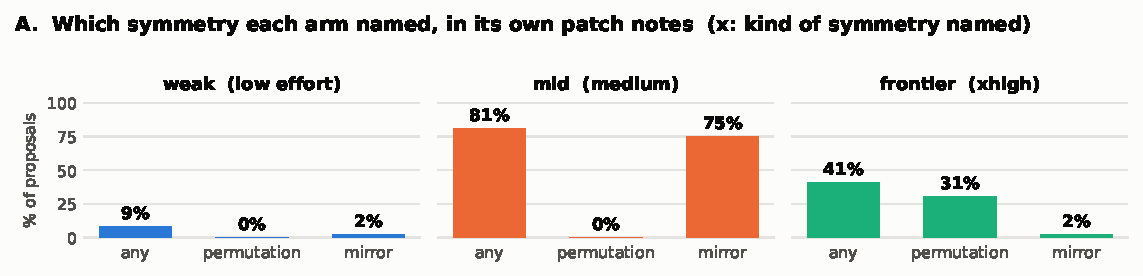
\includegraphics[width=0.505\textwidth]{figA_vocab.pdf}\hfill
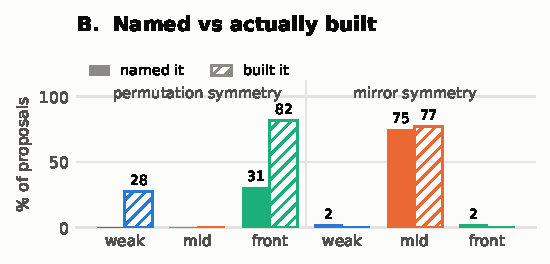
\includegraphics[width=0.238\textwidth]{figB_followthrough.pdf}\hfill
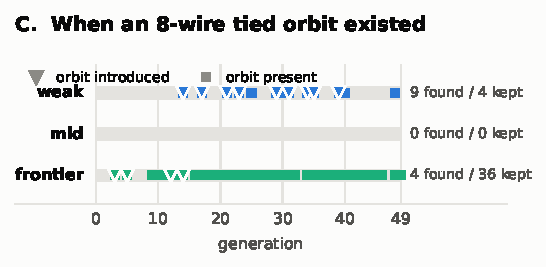
\includegraphics[width=0.243\textwidth]{figC_provenance.pdf}

\vspace{1pt}
{\fontsize{6.4}{7.4}\selectfont\color{inkc}
\textbf{A:} share of each arm's proposals whose patch note uses that vocabulary.
\textbf{B:} solid = named the symmetry, hatched = built the matching structure (8-wire tied
family for permutation; shared $i\,{\leftrightarrow}\,7{-}i$ angle for mirror).
\textbf{C:} squares mark generations whose block contains an 8-wire tied orbit, triangles mark
introductions where the parent lacked it. $n=47$/48/48 proposals with a parseable
ANSATZ\_SPEC. Vocabulary counts detect wording, not understanding; the structural ones do not.\par}

\end{document}
